% !TeX Program=XeLaTeX
% !TeX root = surprises.tex

\selectlanguage{hebrew}


\chapter{משפט חמשת הצבעים}
\label{c.five}

מפות משתמשות בצבעים כדי להבחין בין אזור אחד לאחר, על ידי צביעת אזורים סמוכים בצבעים שונים. בשנת
$1852$
פרנסיס גאת'רי
\L{(Francis Guthrie)}
שם לב שניתן לצבוע את המחוזות באנגליה בארבעה צבעים בלבד. הטענה שארבעה צבעים מספיקים לצביעת כל מפה מישורית נקראת 
\textbf{משפט ארבעת הצבעים}.
המשפט הוכח רק ב-%
$1976$
על ידי קנת אפל
\L{(Kenneth Appel)}
וולפגאנג האקן
\L{(Wolfgang Haken)}.
הם השתמשו במתמטיקה מתקדמת כדי להראות שאם קיימת דוגמה נגדית (מפה הדורשת יותר מארבעה בצבעים), אזי המפה קשורה לאחת מ-%
$1834$
תצורות. לבדיקת התצורות הללו הם השתמשו במחשב.

למרות שקשה מאוד להוכיח את משפט ארבעת הצבעים, ההוכחות של משפט חמשת הצבעים ומשפט ששת הצבעים פשוטות יחסית (סעיפים%
~\ref{s.six-color}, ~\ref{s.five-color}).
בדרך להוכחת משפטים אלו נגדיר מפות מישוריות וגרפים מישוריים (סעיף%
~\ref{s.planar}),
נוכיח את הנוסחה של אוילר 
\L{(Euler)}
(סעיף%
~\ref{s.euler})
ונראה שבגרף מישורי חייב להיות צומת שהדרגה שלו קטנה או שווה לחמש. בסעיף%
~\ref{s.nonplanar}
נשתמש בנוסחת אוילר
כדי להראות ששני גרפים אינם מישוריים.

ב-%
$1879$
פרסם אלפרד קמפ
\L{(Alfred B. Kempe)}
 הוכחה של משפט ארבעת הצבעים וב-%
$1890$
הראה פרסי היווד
\L{(Percy J. Heawood)}
 שההוכחה שגויה. בסעיף%
~\ref{s.kempe}
נביא את ההוכחה השגויה של  קמפ
ואת הדוגמה של
היווד המפריכה את ההוכחה.


\section{מפות מישוריות וגרפים מישוריים}\label{s.planar}

\begin{definition}
\textbf{מפה מישורית}
היא קבוצה של אזורים במישור עם גבולות משותפים.
\textbf{צביעה}
של מפה היא הקצאה של צבע לכל אזור, כך שאזורים בעלי גבול משותף צבועים בצבעים שונים.
\end{definition}
איור%
~\ref{f.five-planar-map-five}
מציג צביעה בחמישה צבעים של מפה מישורית שבה עשרה אזורים. איור%
~\ref{f.five-planar-map-four}
מציג צביעה של אותה מפה בארבעה צבעים. 
\begin{definition}
\textbf{גרף}
הוא קבוצה של 
\textbf{צמתים}
$V$
וקבוצה של 
\textbf{קשתות}
$E$,
כך שכל קשת מחוברת לשני צמתים. הגרף 
\textbf{קשיר}
אם קיים מסלול בין כל שני צמתים.

\textbf{גרף מישורי}
הוא גרף שבו שתי קשתות אינן חותכות זו את זו. בגרף מישורי חלק מהמישור התחום על ידי קבוצה של קשתות נקרא 
\textbf{פאה}.

\textbf{צביעה}
של גרף מישורי היא הקצאה של צבעים לצמתים, כך ששני צמתים המחוברים על ידי קשת צבועים בצבעים שונים.
\end{definition}



\begin{figure}[tb]
\begin{center}
\begin{subfigure}{.4\textwidth}\centering
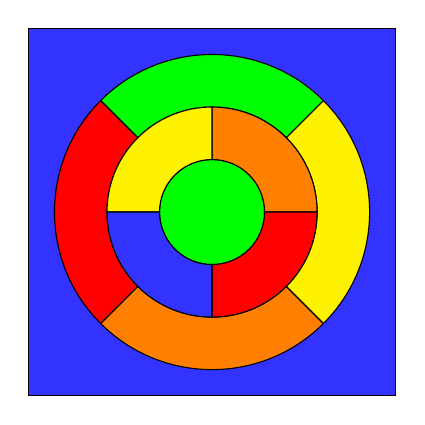
\begin{tikzpicture}[scale=.667]
\draw[fill=blue!80] (-3.5,-3.5) rectangle +(7,7);

\draw[fill=green] (0:1) 
  arc [start angle=0,  end angle=360, radius=1];

\draw[fill=green] (45:2) --
      (45:3)  arc[start angle=45,  end angle=135, radius=3] --
      (135:2) arc[start angle=135, end angle=45,  radius=2];
\draw[fill=orange] (-45:2) --
      (-45:3)  arc[start angle=-45,  end angle=-135, radius=3] --
      (-135:2) arc[start angle=-135, end angle=-45,  radius=2];
\draw[fill=yellow] (45:2) --
      (45:3)  arc[start angle=45,  end angle=-45, radius=3] --
      (-45:2) arc[start angle=-45, end angle=45,  radius=2];
\draw[fill=red] (135:2) --
      (135:3)  arc[start angle=135,  end angle=225, radius=3] --
      (225:2) arc[start angle=225, end angle=135,  radius=2];

\draw[fill=orange] (0:1) --
      (0:2)  arc[start angle=0,  end angle=90, radius=2] --
      (90:1) arc[start angle=90, end angle=0,  radius=1];
\draw[fill=red] (0:1) --
      (0:2)  arc[start angle=0,  end angle=-90, radius=2] --
      (-90:1) arc[start angle=-90, end angle=0,  radius=1];
\draw[fill=yellow] (90:1) --
      (90:2)  arc[start angle=90,  end angle=180, radius=2] --
      (180:1) arc[start angle=180, end angle=90,  radius=1];
\draw[fill=blue!80] (180:1) --
      (180:2)  arc[start angle=180,  end angle=270, radius=2] --
      (270:1) arc[start angle=270, end angle=180,  radius=1];
\end{tikzpicture}
\selectlanguage{hebrew}
\caption{צביעת מפה בחמישה צבעים}\label{f.five-planar-map-five}
\end{subfigure}
\hspace{3em}
\begin{subfigure}{.4\textwidth}\centering
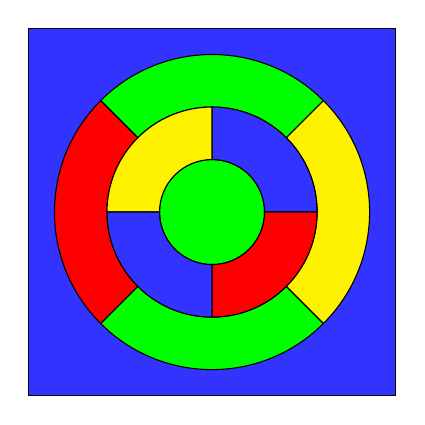
\begin{tikzpicture}[scale=.667]
\draw[fill=blue!80] (-3.5,-3.5) rectangle +(7,7);

\draw[fill=green] (0:1) 
  arc [start angle=0,  end angle=360, radius=1];

\draw[fill=green] (45:2) --
      (45:3)  arc[start angle=45,  end angle=135, radius=3] --
      (135:2) arc[start angle=135, end angle=45,  radius=2];
\draw[fill=green] (-45:2) --
      (-45:3)  arc[start angle=-45,  end angle=-135, radius=3] --
      (-135:2) arc[start angle=-135, end angle=-45,  radius=2];
\draw[fill=yellow] (45:2) --
      (45:3)  arc[start angle=45,  end angle=-45, radius=3] --
      (-45:2) arc[start angle=-45, end angle=45,  radius=2];
\draw[fill=red] (135:2) --
      (135:3)  arc[start angle=135,  end angle=225, radius=3] --
      (225:2) arc[start angle=225, end angle=135,  radius=2];

\draw[fill=blue!80] (0:1) --
      (0:2)  arc[start angle=0,  end angle=90, radius=2] --
      (90:1) arc[start angle=90, end angle=0,  radius=1];
\draw[fill=red] (0:1) --
      (0:2)  arc[start angle=0,  end angle=-90, radius=2] --
      (-90:1) arc[start angle=-90, end angle=0,  radius=1];
\draw[fill=yellow] (90:1) --
      (90:2)  arc[start angle=90,  end angle=180, radius=2] --
      (180:1) arc[start angle=180, end angle=90,  radius=1];
\draw[fill=blue!80] (180:1) --
      (180:2)  arc[start angle=180,  end angle=270, radius=2] --
      (270:1) arc[start angle=270, end angle=180,  radius=1];
\end{tikzpicture}
\selectlanguage{hebrew}
\caption{צביעת מפה בארבעה צבעים}\label{f.five-planar-map-four}
\end{subfigure}
\end{center}
\end{figure}
מפות וגרפים הם דואליים, ונוח יותר לטפל בבעיות צביעה בגרפים מאשר במפות.
\begin{theorem}
נתונה מפה מישורית, ניתן לבנות גרף מישורי כך שעבור כל צביעה של אזורים במפה קיימת צביעה של הצמתים בגרף, ולהפך.
\end{theorem}

\begin{proof}
בנו צומת עבור כל אזור במפה ובנו קשת בין שני צמתים אם ורק אם לשני השטחים יש גבול משותף.
\end{proof}
\begin{example}
איור%
~\ref{f.five-planar-graph-map}
מציג את המפה המישורית מאיור%
~\ref{f.five-planar-map-four}
עם הצמתים המתאימים לכל האזורים. איור%
~\ref{f.five-planar-graph-graph}
מציג גרף מישורי המתאים למפה.
\end{example}

\begin{figure}[tb]
\begin{center}
\begin{subfigure}{.45\textwidth}\centering
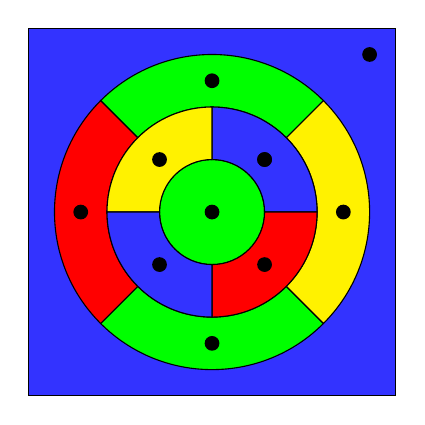
\begin{tikzpicture}[scale=.667]

\draw[fill=blue!80] (-3.5,-3.5) rectangle +(7,7);

\draw[fill=green] (0:1) 
  arc [start angle=0,  end angle=360, radius=1];

\draw[fill=green] (45:2) --
      (45:3)  arc[start angle=45,  end angle=135, radius=3] --
      (135:2) arc[start angle=135, end angle=45,  radius=2];
\draw[fill=green] (-45:2) --
      (-45:3)  arc[start angle=-45,end angle=-135,radius=3] --
      (-135:2) arc[start angle=-135, end angle=-45,  radius=2];
\draw[fill=yellow] (45:2) --
      (45:3)  arc[start angle=45,  end angle=-45, radius=3] --
      (-45:2) arc[start angle=-45, end angle=45,  radius=2];
\draw[fill=red] (135:2) --
      (135:3)  arc[start angle=135,  end angle=225, radius=3] --
      (225:2) arc[start angle=225, end angle=135,  radius=2];

\draw[fill=blue!80] (0:1) --
      (0:2)  arc[start angle=0,  end angle=90, radius=2] --
      (90:1) arc[start angle=90, end angle=0,  radius=1];
\draw[fill=red] (0:1) --
      (0:2)  arc[start angle=0,  end angle=-90, radius=2] --
      (-90:1) arc[start angle=-90, end angle=0,  radius=1];
\draw[fill=yellow] (90:1) --
      (90:2)  arc[start angle=90,  end angle=180, radius=2] --
      (180:1) arc[start angle=180, end angle=90,  radius=1];
\draw[fill=blue!80] (180:1) --
      (180:2)  arc[start angle=180,  end angle=270, radius=2] --
      (270:1) arc[start angle=270, end angle=180,  radius=1];

\foreach \x/\y/\name in {
    0/0/O,
    3/3/Z,
    1/1/E,-1/1/F,-1/-1/G,1/-1/H,
    0/2.5/A,2.5/0/B,0/-2.5/C,-2.5/0/D,
    } {
  \fill (\x,\y) coordinate(\name) circle(4pt);
}
\end{tikzpicture}
\selectlanguage{hebrew}
\caption{התאמת צמתים לאזורים\\
 במפה מישורית}
\label{f.five-planar-graph-map}
\end{subfigure}
\begin{subfigure}{.4\textwidth}\centering
\hspace{2em}
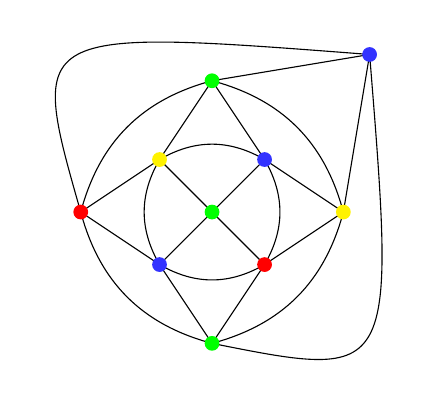
\begin{tikzpicture}[scale=.667]
\foreach \x/\y/\name in {
    0/0/O,
    3/3/Z,
    1/1/E,-1/1/F,-1/-1/G,1/-1/H,
    0/2.5/A,2.5/0/B,0/-2.5/C,-2.5/0/D,
    } {
  \coordinate(\name) at (\x,\y);
}

\draw (E) -- (O) -- (F);
\draw (G) -- (O) -- (H);
\draw (E) to [bend right=30] (F) to [bend right=30] (G) 
          to [bend right=30] (H) to [bend right=30] (E);
\draw (A) -- (E) -- (B) -- (H) -- (C) -- (G) -- (D) -- (F);
\draw (A) to [bend right=30] (D) to [bend right=30] (C) 
          to [bend right=30] (B) to [bend right=30] (A);

\draw (F) -- (A) -- (Z) -- (B);
\draw (C) .. controls (3.5,-3.2) .. (Z);
\draw (D) .. controls (-3.5,3.5) .. (Z);

\foreach \cl/\x/\y in {
    green/0cm/0cm,
    blue!80/3cm/3cm,
    blue!80/1cm/1cm,
    yellow/-1cm/1cm,
    blue!80/-1cm/-1cm,
    red/1cm/-1cm,
    green/0cm/2.5cm,
    yellow/2.5cm/0cm,
    green/0cm/-2.5cm,
    red/-2.5cm/0cm
    }
 \fill[\cl] (\x,\y) circle (4pt);
\end{tikzpicture}
\selectlanguage{hebrew}
\caption{התאמת גרף מישורי\\
למפה המישורית}
\label{f.five-planar-graph-graph}
\end{subfigure}
\end{center}
\end{figure}

ניתן להגביל את עצמנו לגרפים שהפאות שלהם
\textbf{משולשיות}.

\begin{definition}
גרף הוא
\textbf{מתולת
\L{(triangular)}}
אם כל הפאות שלו חסומות על ידי שלוש קשתות. ניתן 
\textbf{לתלת
\L{(triangulate)}}
גרף אם אפשר להוסיף קשתות כדי שהגרף יהי מתולת. נאמר שקיים 
\textbf{תילות
\L{(triangulation)}}
של הגרף.
\end{definition}
\begin{example}
הפאות של הגרף המישורי באיור%
~\ref{f.five-planar-graph-graph}
מתולתות כי כל אחת חסומה על ידי שלוש קשתות. הקשתות עקומות ולכן הפאות אינן משולשים, שהם מצולעים שצלעותיהם קטעים.
\end{example}
\begin{advanced}
משפט
\textbf{F\'{a}ry}
טוען שניתן להמיר כל גרף מישורי מתולת לגרף מישורי שקול שהקשתות שלו הן קטעים. מכאן, שללא הגבלת הכלליות ניתן לנסח הוכחות רק עבור גרפים מישוריים שהפאות שלהם הן משולשים.
\end{advanced}
\begin{example}
איור%
~\ref{f.five-triangular-graph}
(משמאל) מציג ריבוע שניתן לצבוע בשני צבעים, אבל אם מתלתים אותו (במרכז) נדרשים ארבעה צבעים. המטרה שלנו היא להוכיח שניתן לצבוע את כל הגרפים ב-%
$n$
צבעים (עבור
$n$
כלשהו). אם ניתן לצבוע את הגרף המתולת ב- 
$n$
צבעים, אפשר  לצבוע גם את הגרף המקורי באותו מספר צבעים, כי מחיקת הקשתות הנוספות אינו מקלקל את הצביעה (ימין).
\end{example}

\begin{figure}[tb]
\begin{center}
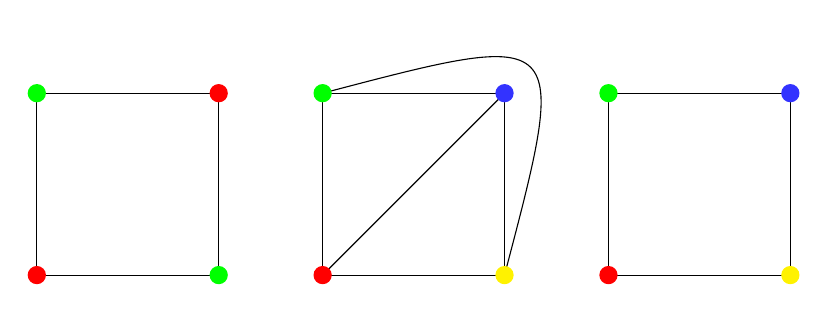
\begin{tikzpicture}[scale=.33]
\draw (-3.5,-3.5) rectangle +(7,7);
\fill[red] (-3.5,-3.5) circle(10pt);
\fill[green] (-3.5,3.5) circle(10pt);
\fill[green] (3.5,-3.5) circle(10pt);
\fill[red] (3.5,3.5) circle(10pt);
\begin{scope}[xshift=11cm]
\draw (-3.5,-3.5) -- (3.5,3.5);
\draw (-3.5,3.5) .. controls (6,6) .. (3.5,-3.5);
\draw (-3.5,-3.5) rectangle +(7,7);
\fill[red] (-3.5,-3.5) circle(10pt);
\fill[green] (-3.5,3.5) circle(10pt);
\fill[yellow] (3.5,-3.5) circle(10pt);
\fill[blue!80] (3.5,3.5) circle(10pt);
\end{scope}
\begin{scope}[xshift=22cm]
\draw (-3.5,-3.5) rectangle +(7,7);
\fill[red] (-3.5,-3.5) circle(10pt);
\fill[green] (-3.5,3.5) circle(10pt);
\fill[yellow] (3.5,-3.5) circle(10pt);
\fill[blue!80] (3.5,3.5) circle(10pt);
\end{scope}
\end{tikzpicture}
\selectlanguage{hebrew}
\caption{צביעת גרף מתולת}\label{f.five-triangular-graph}
\end{center}
\end{figure}

\section{  נוסחת אוילר
\L{\normalsize Euler}}\label{s.euler}

\begin{theorem}[אוילר]\label{thm.euler}
יהי
$G$
גרף מישורי קשיר עם
$V$
צמתים,
$E$
קשתות ו-%
$F$
פאות. אזי:
\[
V-E+F=2\,.
\]
\end{theorem}
\begin{proof}
באינדוקציה על מספר הקשתות. אם מספר הקשתות בגרף מישורי הוא אפס, קיימים רק צומת אחד ופאה אחת כך ש-%
$1-0+1=2$.
אחרת, קיימת לפחות קשת אחת
$e$
שמחברת שני צמתים
$v_1,v_2$.
נמחק את הקשת
$e$.

\textbf{מקרה 1:}
הגרף מפסיק להיות קשיר
(איור~
\ref{f.five-disconnected-removing}).
נמזג את הצמתים
$v_1$
עם
$v_2$
(איור~
\ref{f.five-disconnected-merge}).
נוצר גרף מישורי קשיר
$G'$
 שבו פחות קשתות מאשר ב-%
$G$,
ולכן לפי הנחת האינדוקציה
$(V-1)-(E-1)+F=2$
כי יש בו גם צומת אחד פחות. נפשט ונקבל
$V-E+F=2$
עבור
$G$.

\begin{figure}[tb]
\begin{center}
\begin{subfigure}{.4\textwidth}\centering
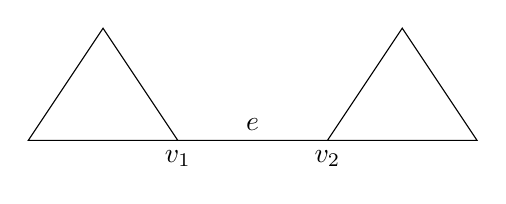
\begin{tikzpicture}[scale=.95]
\draw (2,0) -- (1,1.5) -- (0,0) -- (2,0) node[below] {$v_1$} -- node[above] {$e$} (4,0) node[below] {$v_2$} -- (6,0) -- (5,1.5) -- (4,0);
\end{tikzpicture}
\selectlanguage{hebrew}
\caption{הגרף לא קשיר}\label{f.five-disconnected-removing}
\end{subfigure}
\hspace{3em}
\begin{subfigure}{.4\textwidth}\centering
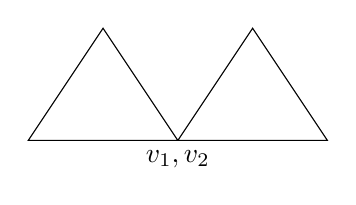
\begin{tikzpicture}[scale=.95]
\draw (2,0) -- (1,1.5) -- (0,0) -- (2,0) node[below] {$v_1,v_2$} -- (4,0) -- (3,1.5) -- (2,0);
\end{tikzpicture}
\selectlanguage{hebrew}
\caption{מיזוג שני צמתים}\label{f.five-disconnected-merge}
\end{subfigure}
\end{center}
\end{figure}

\textbf{מקרה 2:}
הגרף נשאר קשיר
(איור~
\ref{f.five-connected-remains}).
בגרף הנוצר
$G'$
פחות קשתות מאשר ב-%
$G$
(איור~
\ref{f.five-connected-fewer}),
ולכן לפי הנחת האינדוקציה,
$V-(E-1)+(F-1)=2$
מכיוון שמחיקת קשת אחת ממזגת שתי פאות לפאה אחת. נפשט ונקבל
$V-E+F=2$ 
עבור
$G$.
\end{proof}

\begin{figure}[tb]
\begin{center}
\begin{subfigure}{.4\textwidth}\centering
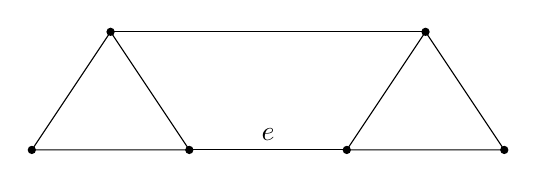
\begin{tikzpicture}
\foreach \x/\y in {0/0, 2/0, 1/1.5,4/0,6/0,5/1.5}
  \fill (\x,\y) circle (1.5pt);
\draw (2,0) -- (1,1.5) -- (0,0) -- (2,0);
\draw (2,0) -- node[above] {$e$} (4,0);
\draw (4,0) -- (6,0) -- (5,1.5) -- (4,0);
\draw (1,1.5) -- (5,1.5);
\end{tikzpicture}
\selectlanguage{hebrew}
\caption{הגרף נשאר קשיר לאחר מחיקת קשת}\label{f.five-connected-remains}
\end{subfigure}
\hspace{3em}
\begin{subfigure}{.4\textwidth}\centering
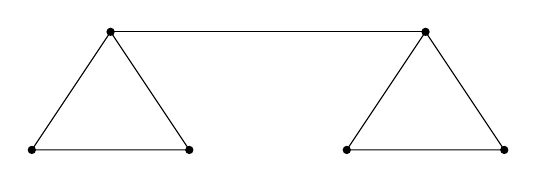
\begin{tikzpicture}
\foreach \x/\y in {0/0, 2/0, 1/1.5,4/0,6/0,5/1.5}
  \fill (\x,\y) circle (1.5pt);
\draw (2,0) -- (1,1.5) -- (0,0) -- (2,0);
\draw (4,0) -- (5,1.5) -- (6,0) -- cycle;
\draw (1,1.5) -- (5,1.5);
\end{tikzpicture}
\selectlanguage{hebrew}
\caption{הגרף קשיר אבל עם פחות קשתות}
\label{f.five-connected-fewer}
\end{subfigure}
\end{center}
\end{figure}

\begin{theorem}\label{thm.edges}
יהי
$G$
גרף מישורי קשיר מתולת עם
$V$
צמתים ו-%
$E$
קשתות. אזי
$E= 3V-6$.
\end{theorem}
\begin{proof}
כל פאה חסומה על ידי שלוש קשתות כך ש-%
$E=3F/2$,
כי כל קשת נספרת פעמיים, פעם אחת לכל פאה שהיא חוסמת. לפי נוסחת אוילר:
\begin{eqn}
E&=&V+F-2\\
E&=&V+2E/3-2\\
E&=&3V-6\,.
\end{eqn}
\end{proof}
\begin{example}
בגרף המישורי באיור%
~\ref{f.five-planar-graph-graph}
יש
$10$
צמתים ו-%
$24= 3\cdot 10-6$
קשתות.
\end{example}
\begin{theorem}\label{thm.count}
יהי
$G$
גרף מישורי קשיר. אז
$E\leq 3V-6$.
\end{theorem}
\begin{proof}
נתלת את
$G$
כדי לקבל את
$G'$.
ב-%
$G'$, $E= 3V-6$
לפי משפט~%
\ref{thm.edges}.
נמחק קשתות מ-%
$G'$
כדי לקבל את
$G$.
מספר הצמתים לא משתנה, כך ש-%
$E\leq 3V-6$.
\end{proof}

\begin{figure}[tb]
\begin{center}
\begin{subfigure}{.45\textwidth}\centering
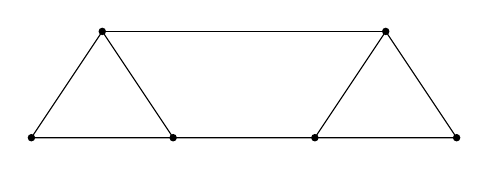
\begin{tikzpicture}[scale=.9]
\foreach \x/\y in {0/0, 2/0, 1/1.5,4/0,6/0,5/1.5}
  \fill (\x,\y) circle (1.5pt);
\draw (2,0) -- (1,1.5) -- (0,0) -- (2,0) -- (4,0) -- (6,0) -- (5,1.5) -- (4,0);
\draw (1,1.5) -- (5,1.5);
\node at (5.5,1) {};
\end{tikzpicture}
\selectlanguage{hebrew}
\caption{פחות קשתות מהחסם העליון}\label{f.five-fewer}
\end{subfigure}
\hspace{1em}
\begin{subfigure}{.45\textwidth}\centering
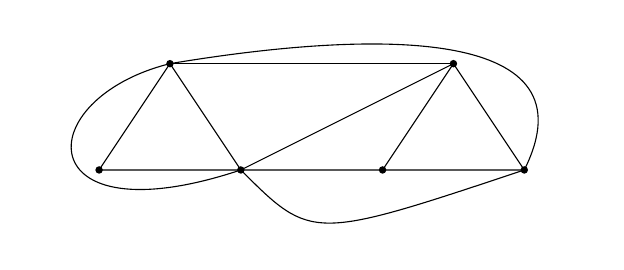
\begin{tikzpicture}[scale=.9]
\foreach \x/\y in {0/0, 2/0, 1/1.5,4/0,6/0,5/1.5}
  \fill (\x,\y) circle (1.5pt);
\draw (2,0) -- (1,1.5) -- (0,0) -- (2,0) -- (4,0) -- (6,0) -- (5,1.5) -- (4,0);
\draw (1,1.5) -- (5,1.5);
\draw (2,0) -- (5,1.5);
\draw (2,0) .. controls (-1,-1) and (-1,1) .. (1,1.5);
\draw (2,0) .. controls (3,-1) .. (6,0) .. controls (7,2) and (4,2) .. (1,1.5);
\end{tikzpicture}
\selectlanguage{hebrew}
\caption{בגרף מתולת מספר הקשתות מירבי}\label{f.five-upper-limit}
\end{subfigure}
\end{center}
\end{figure}
\begin{example}
בגרף ב-%
\ref{f.five-fewer}
$8$
קשתות ו-%
$6$
צמתים ולכן
$8< 3\cdot 6 - 6= 12$.
איור%
~\ref{f.five-upper-limit}
מציג גרף מתולת עם
$6$
צמתים ו-%
$3\cdot 6 - 6= 12$
קשתות.
\end{example}

\section{גרפים שאינם מישוריים}
נסטה מעט מהסיפור כדי להראות איך ניתן להשתמש במשפטים% 
~\ref{thm.euler}\label{s.nonplanar}
ו-%
\ref{thm.count}
כדי להוכיח שגרפים מסוימים אינם מישוריים.

\begin{theorem}
$K_5$,
הגרף השלם עם חמישה צמתים, אינו מישורי 
(איור%
~\ref{f.five-k5-failed}).
\end{theorem}
\begin{figure}[tb]
\begin{center}
\begin{subfigure}{.45\textwidth}\centering
\begin{tikzpicture}[scale=.75]
\node (pentagon) [minimum size=4cm,regular polygon,regular polygon sides=5] at (0,0) {};
\draw (pentagon.corner 1) -- (pentagon.corner 2);
\draw (pentagon.corner 2) -- (pentagon.corner 3);
\draw (pentagon.corner 3) -- (pentagon.corner 4);
\draw (pentagon.corner 4) -- (pentagon.corner 5);
\draw (pentagon.corner 5) -- (pentagon.corner 1);
\draw (pentagon.corner 1) -- (pentagon.corner 3);
\draw (pentagon.corner 1) -- (pentagon.corner 4);
\draw (pentagon.corner 2) -- (pentagon.corner 4);
\draw (pentagon.corner 2) -- (pentagon.corner 5);
\draw (pentagon.corner 3) -- (pentagon.corner 5);
\node at (4,2) {};
\end{tikzpicture}
\selectlanguage{hebrew}
\caption{$K_5$
אינו מישורי}
\label{f.five-k5-failed}
\end{subfigure}
\hspace{1em}
\begin{subfigure}{.45\textwidth}\centering
\begin{tikzpicture}[scale=.75]
\node (pentagon) [minimum size=4cm,regular polygon,regular polygon sides=5] at (0,0) {};
\draw (pentagon.corner 1) -- (pentagon.corner 2);
\draw (pentagon.corner 2) -- (pentagon.corner 3);
\draw (pentagon.corner 3) -- (pentagon.corner 4);
\draw (pentagon.corner 4) -- (pentagon.corner 5);
\draw (pentagon.corner 5) -- (pentagon.corner 1);
\draw (pentagon.corner 1) .. controls (-4,1) .. 
      (pentagon.corner 3);
\draw (pentagon.corner 1) .. controls (4,1) ..
      (pentagon.corner 4);
\draw (pentagon.corner 2) -- (pentagon.corner 4);
\draw (pentagon.corner 2) -- (pentagon.corner 5);
\draw (pentagon.corner 3) -- (pentagon.corner 5);
\draw[thick] (0,-.75) circle(5pt);
\end{tikzpicture}
\selectlanguage{hebrew}
\caption{$K_5$
אינו מישורי
}\label{f.k5}
\end{subfigure}
\end{center}
\end{figure}
\begin{proof}
עבור
$K_5$, $V=5$
ו-%
$E=10$.
לפי משפט%
~\ref{thm.count}
מספר הקשתות חייב להיות קטן או שווה ל-%
$3\cdot 5 -6=9$
ולכן הגרף אינו מישורי.
\end{proof}
\begin{theorem}
$K_{3,3}$,
הגרף הדו-אזורי עם שלושה צמתים בכל אזור 
(איור~
\ref{f.five-k33}),
אינו מישורי.
\end{theorem}
\begin{figure}[tb]
\begin{center}
\begin{subfigure}{.4\textwidth}\centering
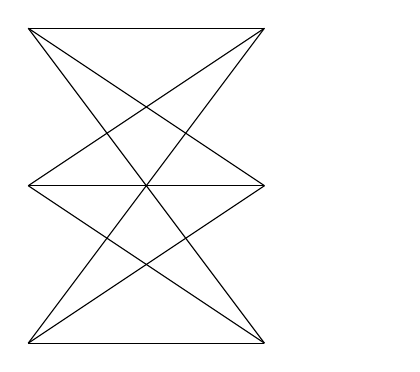
\begin{tikzpicture}[scale=1]
\draw (0,0) -- (3,0);
\draw (0,2) -- (3,2);
\draw (0,4) -- (3,4);
\draw (0,0) -- (3,2);
\draw (0,2) -- (3,4);
\draw (0,4) -- (3,0);
\draw (0,0) -- (3,4);
\draw (0,2) -- (3,0);
\draw (0,4) -- (3,2);
\node at (4.5,1) {};
\end{tikzpicture}
\selectlanguage{hebrew}
\caption{$K_{3,3}$ אינו מישורי}\label{f.five-k33}
\end{subfigure}
\hspace{3em}
\begin{subfigure}{.4\textwidth}\centering
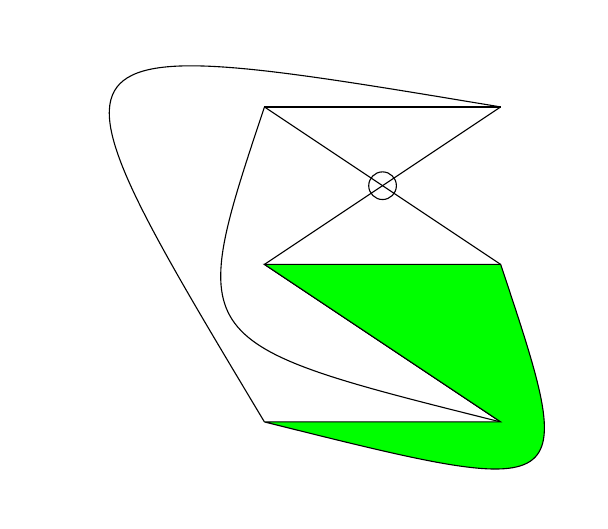
\begin{tikzpicture}
\draw (0,4) -- (3,4);
\draw (0,2) -- (3,4);
\draw (0,4) .. controls (-1,1) .. (3,0);
\draw (0,0) .. controls (-3,5) .. (3,4);
\draw (0,2) -- (3,0);
\draw (0,4) -- (3,2);
\draw[fill=green] (0,0) -- (3,0) -- (3,0) -- (0,2)  -- (3,2) .. controls (4,-1) .. (0,0);
\draw (1.5,3) circle(5pt);
\end{tikzpicture}
\selectlanguage{hebrew}
\caption{ניסיון כושל לצייר את
$K_{3,3}$
במישור}
\label{f.five-k33-failed}
\end{subfigure}
\end{center}
\end{figure}
\begin{proof}
$V=6$
ו-%
$E=9$.
לפי משפט%
~\ref{thm.euler},
אם
$K_{3,3}$
מישורי,
$F=E-V+2=9-6+2=5$.
אבל כל פאה חסומה על ידי ארבע קשתות
(איור \ref{f.five-k33-failed}),
ולכן
$E=4F/2=(4\cdot 5)/2\neq 9$.
\end{proof}

 בשנת הוכיח קזימירייז קורטובסקי
$1930$
\L{(Kazimierz Kuratowski)}
 את הכיוון השני של המשפטים הללו: אם גרף אינו מישורי, אז הוא מכיל (במובן מסוים) 
$K_5$
או
$K_{3,3}$.

%%%%%%%%%%%%%%%%%%%%%%%%%%%%%%%%%%%%%%%%%%%%%%%%%%%

\section{דרגה של צמתים}\label{s.degrees}

\begin{definition}
$d(v)$,
\textbf{הדרגה}
של צומת
$v$,
היא מספר הקשתות הנפגשות ב-%
$v$.
\end{definition}

\begin{example}
בגרף באיור%
~\ref{f.five-planar-graph-graph}
$8$
צמתים על שתי הטבעות, כל אחד מדרגה
$5$.
ושני צמתים נוספים, על הפאה החיצונית ועל הפאה הפנימית, שדרגתם   
$4$.
לכן:
\[
\sum_{v\in V} d(v) = 5\cdot 8 + 4\cdot 2=48\,.
\]
לקבלת מספר הקשתות בגרף נחלק את סכום הדרגות ב-%
$2$,
כי כל קשת נספרה פעמיים, פעם אחת עבור כל צומת שהיא נוגעת בו.
\end{example}
הכללת הטיעונים הללו מוכיחה:
\begin{theorem}\label{thm.degrees}
יהי
$d_i, i=1,2,3,\ldots,k$
מספרי הצמתים מדרגה
$i$
בגרף מישורי קשיר עם
$V$
צמתים ו-%
$E$ 
קשתות, כאשר
$k$
היא הדרגה הגבוהה ביותר של צומת ב-%
$V$.
אז:
\[
\sum_{v\in V} d(v) =\sum_{i=1}^{k} i\cdot d_i=2E\,.
\]
\end{theorem}
\begin{theorem}\label{thm.degree5}
יהי
$G$
גרף מישורי קשיר עם
$E$
קשתות ו-%
$V$
צמתים, ויהי
$d_i,i=1,\ldots,k$
מספר ההצמתים מדרגה
$i$,
כאשר
$k$
היא הדרגה הגבוהה ביותר של צומת ב-%
$V$.
אזי חייב להיות צומת
$v$
ב-%
$V$
כך ש-%
$d(v) \leq 5$.
\end{theorem}
\begin{proof}
\textbf{(1)}
ברור שאם יש 
$d_1$
צמתים מדרגה
$1$, $d_2$ 
צמתים מדרגה
$2$, \ldots, $d_k$
צמתים מדרגה
$k$, 
אז
$V=\sum_{i=1}^{k}d_i$. 
ממשפטים%
~\ref{thm.count}
ו-%
\ref{thm.degrees}
נקבל:
\[
\sum_{i=1}^{k} i\cdot d_i=2E\leq 2(3V-6) = 6V-12=6\sum_{i=1}^{k} d_i -12\,.
\]
מכאן,
\begin{eqn}
\sum_{i=1}^{k} i\cdot d_i \leq 6\sum_{i=1}^{k} d_i -12\\
\sum_{i=1}^{k} (6-i)d_i\geq 12\,.
\end{eqn}
$12>0$,
ולכן ל-%
$i$
אחד לפחות מתקיים
$6-i>0$
ועבור 
$i$
זה,
$i<6$. 
\end{proof}

\begin{proof}
\textbf{(2)}
נחשב את 
\textbf{הממוצע}
של דרגות הצמתים, שהוא סכום הדרגות לחלק למספר הצמתים:
\[
d_{\textit{\footnotesize avg}}=\frac{\sum_{i=1}^{k} i\cdot d_i}{V}\,.
\]
אבל סכום הדרגות הוא פעמיים מספר הקשתות, ולפי משפט%
~\ref{thm.count}:
\[
d_{\textit{\footnotesize avg}}=\frac{2E}{V}\leq \frac{6V-12}{V}=6-\frac{6}{V}<6\,.
\]
אם 
\textbf{הממוצע}
של הדרגות קטן משש, חייב להיות לפחות צומת אחד שדרגתו קטנה משש.
\end{proof}

\begin{example}
סכום הדרגות בגרף באיור%
~\ref{f.five-planar-graph-graph}
הוא
$8\cdot 5 + 2\cdot 4=48$.
יש 
$10$
צמתים כך שממוצע הדרגות שלו הוא
$48/10=4.8$
וחייב להיות צומת ממעלה 
$4$
או פחות.
\end{example}

\section{משפט ששת הצבעים}\label{s.six-color}

\begin{theorem}\label{thm.sixcolor}
כל גרף מישורי ניתן לצביעה בשישה צבעים.
\end{theorem}

\begin{proof}
באינדוקציה על מספר הצמתים ב-%
$G$.
אם בגרף שישה צמתים או פחות, ברור שניתן לצבוע את הגרף בשישה צבעים. עבור הצעד האינדוקטיבי, לפי משפט
~\ref{thm.degree5}
קיים צומת
$v$
מדרגה חמש או פחות. נמחק צומת
$v$
כדי לקבל את הגרף
$G'$.
לפי הנחת האינדוקציה ניתן לצבוע את
$G'$
בשישה צבעים, אבל ל-%
$v$
חמישה שכנים לכל היותר והם צבועים בחמישה צבעים לכל היותר
(איור~%
\ref{f.five-six-five}),
כך שנשאר צבע שישי שניתן לצבוע בו את
$v$
(איור~%
\ref{f.five-six-six}).
\end{proof}

\begin{figure}[tb]
\begin{center}
\begin{subfigure}{.4\textwidth}\centering
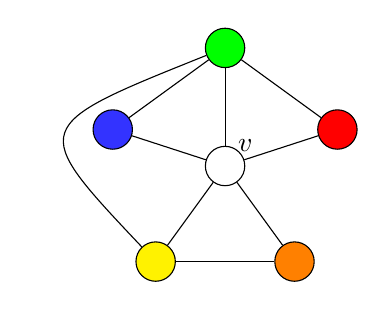
\begin{tikzpicture}[scale=.5,minimum size=5mm,inner sep=0pt]
\foreach \name/\color/\theta in
    {A/red/18,B/green/90,C/blue!80/162,D/yellow/234,E/orange/306}
  \node[circle,draw,fill=\color] (\name) at (\theta:3) {};
\node[circle,draw] (O) at (0,0) {};
\node[above right] at (O) {$v$};
\foreach \name in {A,B,C,D,E}
  \draw (O) -- (\name);
\foreach \i/\j in {A/B,B/C,D/E}
  \draw (\i) -- (\j);
\draw (B) .. controls (-5,1) .. (D);
\end{tikzpicture}
\selectlanguage{hebrew}
\caption{חמישה צבעים מספיקים לשכנים של
$v$}\label{f.five-six-five}
\end{subfigure}
\hspace{3em}
\begin{subfigure}{.4\textwidth}\centering
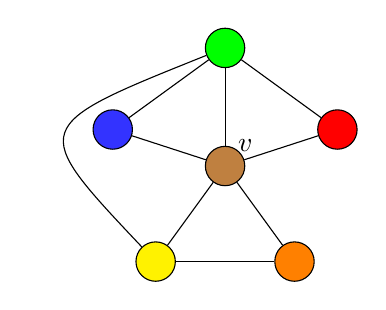
\begin{tikzpicture}[scale=.5,minimum size=5mm,inner sep=0pt]
\foreach \name/\color/\theta in
    {A/red/18,B/green/90,C/blue!80/162,D/yellow/234,E/orange/306}
  \node[circle,draw,fill=\color] (\name) at (\theta:3) {};
\node[circle,draw,fill=brown] (O) at (0,0) {};
\node[above right] at (O) {$v$};
\foreach \name in {A,B,C,D,E}
  \draw (O) -- (\name);
\foreach \i/\j in {A/B,B/C,D/E}
  \draw (\i) -- (\j);
\draw (B) .. controls (-5,1) .. (D);
\end{tikzpicture}
\selectlanguage{hebrew}
\caption{נצבע את
$v$
בצבע השישי}
\label{f.five-six-six}
\end{subfigure}
\end{center}
\end{figure}

\section{משפט חמשת הצבעים}\label{s.five-color}

\begin{definition}
יהי
$G$
גרף מישורי קשיר צבוע. 
$G'$
הוא
\textbf{שרשרת}
אם ורק אם
$G'$
הוא תת-גרף מקסימלי של
$G$
הצבוע בשני צבעים.%
\footnote{%
השרשרת נקראת גם שרשרת קמפ
כי היא הוגדרה על ידי אלפרד קמפ
בהוכחה השגויה שלו למשפט ארבעת הצבעים.}
\end{definition}
\begin{theorem}\label{thm.fivecolor}
כל גרף מישורי 
$G$
ניתן לצביעה בחמישה צבעים.
\end{theorem}

\begin{proof}
באינדקציה על מספר הצמתים. אם ב-%
$G$
חמישה צמתים או פחות, ניתן לצבוע אותו בחמישה צבעים. עבור הצעד האינדוקטיבי, לפי משפט%
~\ref{thm.degree5}
קיים צומת
$v$
מדרגה חמש או פחות. נמחק את הצומת
$v$
ונקבל את הגרף
$G'$.
לפי הנחת האינדוקציה, ניתן לצבוע את
$G'$
בחמישה צבעים או פחות. ב-%
$G$,
אם הדרגה של
$v$
קטנה מחמש, או אם
$v_1,\ldots,v_5$,
השכנים של
$v$,
צבועים בארבעה צבעים או פחות, ניתן לצבוע את
$v$
בצבע החמישי. אחרת, הצמתים
$v_1,\ldots,v_5$
צבועים בצבעים שונים ב-%
$G'$
(איור%
~\ref{f.five-color-proof},
למעלה).
\begin{figure}[tb]
\begin{center}
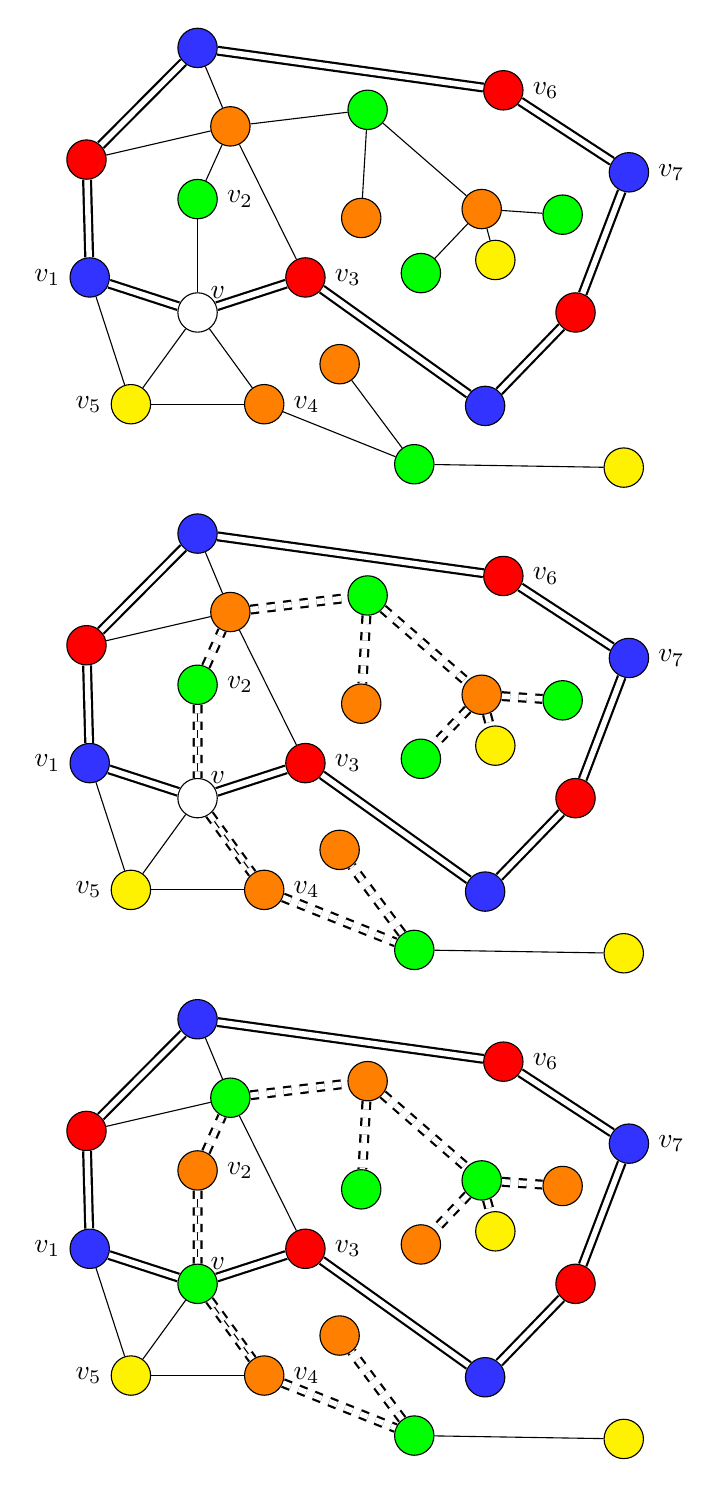
\begin{tikzpicture}[scale=.48,minimum size=5mm,inner sep=0pt]
\foreach \name/\color/\theta in
    {A/red/18,B/green/90,C/blue!80/162,D/yellow/234,E/orange/306}
  \node[circle,draw,fill=\color] (\name) at (\theta:3) {};
\node[circle,draw] (O) at (0,0) {};
\node[above right] at (O) {$v$};

\node[right,xshift=8pt] at (A) {$v_3$};
\node[right,xshift=8pt] at (B) {$v_2$};
\node[left,,xshift=-8pt] at (C) {$v_1$};
\node[left,,xshift=-8pt] at (D) {$v_5$};
\node[right,xshift=8pt] at (E) {$v_4$};

\foreach \name in {A,B,C,D,E}
  \draw (O) -- (\name);
  
\node[circle,draw,fill=red]  (X1) at (126:5) {};
\node[circle,draw,fill=blue!80] (X2) at (90:7)  {};
\node[circle,draw,fill=red]  (X3) at (36:10) {};
\node[right,xshift=8pt] at (X3) {$v_6$};
\node[circle,draw,fill=blue!80] (X4) at (18:12) {};
\node[right,xshift=8pt] at (X4) {$v_7$};
\node[circle,draw,fill=red]  (X5) at (0:10) {};
\node[circle,draw,fill=blue!80] (X6) at (-18:8) {};
\draw[thick,double distance=2pt] (C)  -- (X1);
\draw[thick,double distance=2pt] (X1) -- (X2);
\draw[thick,double distance=2pt] (X2) -- (X3);
\draw[thick,double distance=2pt] (X3) -- (X4);
\draw[thick,double distance=2pt] (X4) -- (X5);
\draw[thick,double distance=2pt] (X5) -- (X6);
\draw[thick,double distance=2pt] (X6) -- (A);
\draw[thick,double distance=2pt] (A) -- (O) -- (C);

\node[circle,draw,fill=orange]  (Y1)  at (80:5) {};
\node[circle,draw,fill=green]   (Y2)  at (50:7)  {};
\node[circle,draw,fill=orange]  (Y3A) at (20:8) {};
\node[circle,draw,fill=orange]  (Y3B) at (30:5) {};
\node[circle,draw,fill=green]   (Y4A) at (10:6) {};
\node[circle,draw,fill=yellow]  (Y4B) at (10:8) {};
\node[circle,draw,fill=green]   (Y4C) at (15:10) {};
\node[circle,draw,fill=green]   (Y5)  at (-35:7) {};
\node[circle,draw,fill=yellow]  (Y6A) at (-20:12) {};
\node[circle,draw,fill=orange]  (Y6B) at (-20:4) {};
\draw (B)  -- (Y1);
\draw (Y1) -- (Y2);
\draw (Y2) -- (Y3A);
\draw (Y2) -- (Y3B);
\draw (Y3A) -- (Y4A);
\draw (Y3A) -- (Y4B);
\draw (Y3A) -- (Y4C);
\draw (E)  -- (Y5);
\draw (Y5) -- (Y6A);
\draw (Y5) -- (Y6B);
\draw (A) -- (Y1);
\draw (X2) -- (Y1);
\draw (X1) -- (Y1);
\draw (D) -- (E);
\draw (D) -- (C);

\begin{scope}[yshift=-12.85cm]
\foreach \name/\color/\theta in
    {A/red/18,B/green/90,C/blue!80/162,D/yellow/234,E/orange/306}
  \node[circle,draw,fill=\color] (\name) at (\theta:3) {};
\node[circle,draw] (O) at (0,0) {};
\node[above right] at (O) {$v$};

\node[right,xshift=8pt] at (A) {$v_3$};
\node[right,xshift=8pt] at (B) {$v_2$};
\node[left,,xshift=-8pt] at (C) {$v_1$};
\node[left,,xshift=-8pt] at (D) {$v_5$};
\node[right,xshift=8pt] at (E) {$v_4$};

\foreach \name in {A,B,C,D,E}
  \draw (O) -- (\name);
  
\node[circle,draw,fill=red]  (X1) at (126:5) {};
\node[circle,draw,fill=blue!80] (X2) at (90:7)  {};
\node[circle,draw,fill=red]  (X3) at (36:10) {};
\node[circle,draw,fill=blue!80] (X4) at (18:12) {};
\node[circle,draw,fill=red]  (X5) at (0:10) {};
\node[circle,draw,fill=blue!80] (X6) at (-18:8) {};

\draw[thick,double distance=2pt] (C)  -- (X1);
\draw[thick,double distance=2pt] (X1) -- (X2);
\draw[thick,double distance=2pt] (X2) -- (X3);
\draw[thick,double distance=2pt] (X3) -- (X4);
\draw[thick,double distance=2pt] (X4) -- (X5);
\draw[thick,double distance=2pt] (X5) -- (X6);
\draw[thick,double distance=2pt] (X6) -- (A);
\draw[thick,double distance=2pt] (A) -- (O) -- (C);

\node[circle,draw,fill=orange]  (Y1)  at (80:5) {};
\node[circle,draw,fill=green]   (Y2)  at (50:7)  {};
\node[circle,draw,fill=orange]  (Y3A) at (20:8) {};
\node[circle,draw,fill=orange]  (Y3B) at (30:5) {};
\node[circle,draw,fill=green]   (Y4A) at (10:6) {};
\node[circle,draw,fill=yellow]   (Y4B) at (10:8) {};
\node[circle,draw,fill=green]   (Y4C) at (15:10) {};
\node[circle,draw,fill=green]   (Y5)  at (-35:7) {};
\node[circle,draw,fill=yellow]  (Y6A) at (-20:12) {};
\node[circle,draw,fill=orange]  (Y6B) at (-20:4) {};
\draw[thick,dashed,double distance=2pt] (B)  -- (O) -- (E);
\draw[thick,dashed,double distance=2pt] (B)  -- (Y1);
\draw[thick,dashed,double distance=2pt] (Y1) -- (Y2);
\draw[thick,dashed,double distance=2pt] (Y2) -- (Y3A);
\draw[thick,dashed,double distance=2pt] (Y2) -- (Y3B);
\draw[thick,dashed,double distance=2pt] (Y3A) -- (Y4A);
\draw[thick,dashed,double distance=2pt] (Y3A) -- (Y4B);
\draw[thick,dashed,double distance=2pt] (Y3A) -- (Y4C);
\draw[thick,dashed,double distance=2pt] (E)  -- (Y5);
\draw[thick,dashed,double distance=2pt] (Y5) -- (Y6B);
\draw (Y5) -- (Y6A);
\draw (A) -- (Y1);
\draw (X2) -- (Y1);
\draw (X1) -- (Y1);
\draw (D) -- (E);
\draw (D) -- (C);
\node[right,xshift=8pt] at (X3) {$v_6$};
\node[right,xshift=8pt] at (X4) {$v_7$};
\end{scope}

\begin{scope}[yshift=-25.7cm]
\foreach \name/\color/\theta in
    {A/red/18,B/orange/90,C/blue!80/162,D/yellow/234,E/orange/306}
  \node[circle,draw,fill=\color] (\name) at (\theta:3) {};
\node[circle,draw,fill=green] (O) at (0,0) {};
\node[above right] at (O) {$v$};

\node[right,xshift=8pt] at (A) {$v_3$};
\node[right,xshift=8pt] at (B) {$v_2$};
\node[left,,xshift=-8pt] at (C) {$v_1$};
\node[left,,xshift=-8pt] at (D) {$v_5$};
\node[right,xshift=8pt] at (E) {$v_4$};

\foreach \name in {A,B,C,D,E}
  \draw (O) -- (\name);
  
\node[circle,draw,fill=red]  (X1) at (126:5) {};
\node[circle,draw,fill=blue!80] (X2) at (90:7)  {};
\node[circle,draw,fill=red]  (X3) at (36:10) {};
\node[circle,draw,fill=blue!80] (X4) at (18:12) {};
\node[circle,draw,fill=red]  (X5) at (0:10) {};
\node[circle,draw,fill=blue!80] (X6) at (-18:8) {};

\draw[thick,double distance=2pt] (C)  -- (X1);
\draw[thick,double distance=2pt] (X1) -- (X2);
\draw[thick,double distance=2pt] (X2) -- (X3);
\draw[thick,double distance=2pt] (X3) -- (X4);
\draw[thick,double distance=2pt] (X4) -- (X5);
\draw[thick,double distance=2pt] (X5) -- (X6);
\draw[thick,double distance=2pt] (X6) -- (A);
\draw[thick,double distance=2pt] (A) -- (O) -- (C);

\node[circle,draw,fill=green]  (Y1)  at (80:5) {};
\node[circle,draw,fill=orange]   (Y2)  at (50:7)  {};
\node[circle,draw,fill=green]  (Y3A) at (20:8) {};
\node[circle,draw,fill=green]  (Y3B) at (30:5) {};
\node[circle,draw,fill=orange]   (Y4A) at (10:6) {};
\node[circle,draw,fill=yellow]   (Y4B) at (10:8) {};
\node[circle,draw,fill=orange]   (Y4C) at (15:10) {};
\node[circle,draw,fill=green]   (Y5)  at (-35:7) {};
\node[circle,draw,fill=yellow]  (Y6A) at (-20:12) {};
\node[circle,draw,fill=orange]  (Y6B) at (-20:4) {};

\draw[thick,dashed,double distance=2pt] (B)  -- (O) -- (E);
\draw[thick,dashed,double distance=2pt] (B)  -- (Y1);
\draw[thick,dashed,double distance=2pt] (Y1) -- (Y2);
\draw[thick,dashed,double distance=2pt] (Y2) -- (Y3A);
\draw[thick,dashed,double distance=2pt] (Y2) -- (Y3B);
\draw[thick,dashed,double distance=2pt] (Y3A) -- (Y4A);
\draw[thick,dashed,double distance=2pt] (Y3A) -- (Y4B);
\draw[thick,dashed,double distance=2pt] (Y3A) -- (Y4C);
\draw[thick,dashed,double distance=2pt] (E)  -- (Y5);
\draw[thick,dashed,double distance=2pt] (Y5) -- (Y6B);


\draw (Y5) -- (Y6A);
\draw (A) -- (Y1);
\draw (X2) -- (Y1);
\draw (X1) -- (Y1);
\draw (D) -- (E);
\draw (D) -- (C);
\node[right,xshift=8pt] at (X3) {$v_6$};
\node[right,xshift=8pt] at (X4) {$v_7$};
\end{scope}
\end{tikzpicture}
\end{center}
\selectlanguage{hebrew}
\caption{הוכחת משפט חמשת הצבעים}\label{f.five-color-proof}
\end{figure}

נתבונן בצומת
$v_1$
הצבוע בכחול ובצומת 
$v_3$
צבוע באדום. אם
$v_1,v_3$
לא קשורים במסלול כחול-אדום (למשל, אם הקשת 
$\overline{v_6v_7}$
לא הייתה קיימת), ניתן להחליף את הצבעים על המסלול מ-%
$v_1$
ל-%
$v_6$
ולצבוע את 
$v$
בכחול. אחרת, ניקח את שרשרת הכחול-אדום המכילה את
$v_1,v_3$
ונוסיף את
$v$
ואת הקשתות
$\overline{vv_1},\overline{vv_3}$.
נקבל מסלול סגור
$P$
(המסומן בקו כפול) שמחלק את המישור לאזור "פנימי" ולאזור "חיצוני" (איור%
~\ref{f.five-color-proof}, \R{אמצע}).

\newpage

כעת נתבונן בצומת
$v_2$
הצבוע ירוק ובצומת
$v_4$
הצבוע כתום. הצמתים הללו 
\textbf{אינם}
יכולים להיות בשרשרת ירוק-כתום אחת, כי 
$v_2$
נמצא 
\textbf{בתוך}
$P$
ו-%
$v_4$
נמצא
\textbf{מחוץ}
ל-%
$P$,
ולכן כל מסלול המחבר אותם חייב לחתוך את
$P$,
בסתירה להנחה שהגרף מישורי. לכן הם חייבים להיות בתוך שתי שרשראות ירוק-כתום 
\textbf{לא קשורות}
(מסומנות בקו מקווקוו כפול באיור
~\ref{f.five-color-proof}, \R{באמצע}).
נחליף את שני הצבעים בשרשרת המכילה את
$v_2$
ואז אפשר לצבוע את 
$v$
בירוק כדי לקבל צביעה של 
$G$
בחמישה צבעים (איור%
~\ref{f.five-color-proof}, \R{למטה}).
\end{proof}

%%%%%%%%%%%%%%%%%%%%%%%%%%%%%%%%%%%%%%%%%%%%%%%%%%%%%%%%%%%

\begin{advanced}
הטענה שמסלול רציף מתוך עקומה רציפה סגורה 
$P$
אל מחוץ ל-%
$P$
חייב לחתוך את
$P$
היא משפט העקום של ז'ורדן 
\L{\textbf{(Jordan Curve Theorem)}}.
המשפט ברור אינטואיטיבית אבל קשה להוכחה.
\end{advanced}

%%%%%%%%%%%%%%%%%%%%%%%%%%%%%%%%%%%%%%%%%%%%%%%%%%%%%%%%%%%

\section{ההוכחה השגויה של קמפ לבעיית ארבעת הצבעים}
\label{s.kempe}

\begin{proof}
\textbf{(שגויה)}
בסיס האינדוקציה ורוב ההוכחה זהים להוכחה של משפט חמשת הצבעים. המקרה החדש שיש לקחת בחשבון הוא צומת 
$v$
עם חמישה שכנים, שלפי ההנחה האינדוקטיבית ניתן לצבוע אותם
\textbf{בארבעה}
צבעים לאחר מחיקת הצומת
$v$.

ב-%
\ref{f.five-kempe1}
קיימים שני צמתים
$v_2,v_5$
הצבועים בכחול. נתבונן בשרשרת הכחול-ירוק המכילה את 
$v_2$
ובשרשרת הכחול-צהוב המכילה את
$v_5$.
השרשרת הכחול-ירוק נמצאת מתוך המסלול הסגור המוגדר על ידי השרשרת האדום-צהוב שמכילה את
$v_1,v_3$
(מסומן בקו כפול), והשרשרת הכחול-צהוב נמצאת בתוך המסלול הסגור המוגדר על ידי השרשרת האדום-ירוק המכילה את
$v_1,v_4$
(מסומן בקו כפול מקווקוו).

נחליף את הצבעים בשתי השרשרות, שרשרת הכחול-ירוק ושרשרת הכחול-צהוב 
(איור%
~\ref{f.five-kempe1-exchange}).
השכנים של
$v$
צבועים בשלושה צבעים, אדום, ירוק וצהוב, וניתן לצבוע את
$v$
בכחול.
\end{proof}


\begin{figure}[tb]
\begin{center}
\begin{subfigure}{.4\textwidth}
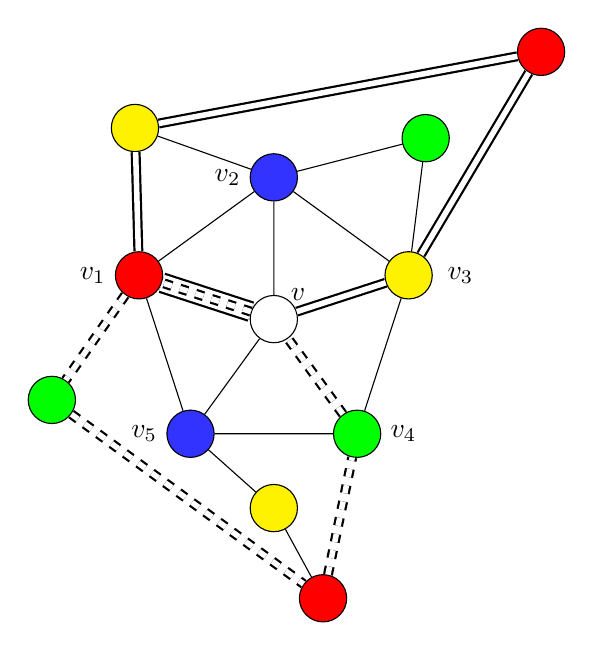
\begin{tikzpicture}[scale=.6,minimum size=6mm,inner sep=0pt]

% Draw center node and adjacent nodes
\foreach \name/\color/\theta in
    {A/yellow/18,B/blue!80/90,C/red/162,D/blue!80/234,E/green/306}
  \node[circle,draw,fill=\color] (\name) at (\theta:3) {};
\node[circle,draw] (O) at (0,0) {};
\node[above right]     at (O) {$v$};

\node[right,xshift=10pt] at (A) {$v_3$};
\node[left,xshift=-8pt]  at (B) {$v_2$};
\node[left,xshift=-8pt]  at (C) {$v_1$};
\node[left,xshift=-8pt]  at (D) {$v_5$};
\node[right,xshift=8pt]  at (E) {$v_4$};

% Draw red-yellow path
\node[circle,draw,fill=yellow]  (X1) at (126:5) {};
\node[circle,draw,fill=red] (X2) at (45:8)  {};

\draw[thick,double distance=2pt] 
  (C) -- (X1) -- (X2) -- (A) -- (O);
\draw[thick,double distance=6pt] (O) -- (C);

% Draw blue-green nodes within red-yellow path
\node[circle,draw,fill=green] (Y1)  at (50:5) {};

% Draw red-green path
\node[circle,draw,fill=green] (Z1)  at (-160:5) {};
\node[circle,draw,fill=red]   (Z2)  at (-80:6)  {};

%\draw[thick,dashed,double distance=6pt] (O) -- (C);
\draw[thick,dashed,double distance=2pt] 
  (O) -- (C) -- (Z1) -- (Z2) -- (E) -- (O);

% Draw blue-yellow nodes within red-green path
\node[circle,draw,fill=yellow]   (U1)  at (-90:4)  {};

% Connect adjacent nodes not in paths
\draw (X1) -- (B) -- (Y1) -- (A) -- (B) -- 
      (C) -- (D) -- (E) -- (A);
\draw (Z2) -- (U1) -- (D) -- (O) -- (B);

\end{tikzpicture}
\selectlanguage{hebrew}
\caption{שרשארות
\L{Kempe}
ירוק-כחול וכחול-צהוב}
\label{f.five-kempe1}
\end{subfigure}
\hspace{3em}
\begin{subfigure}{.4\textwidth}
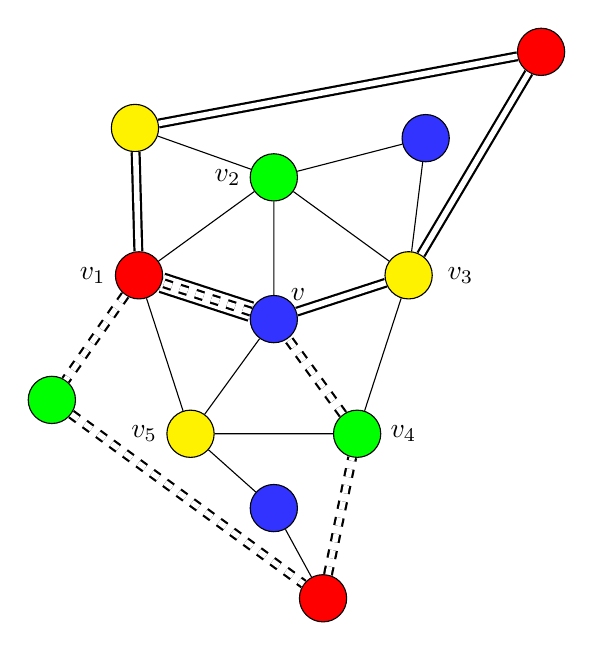
\begin{tikzpicture}[scale=.6,minimum size=6mm,inner sep=0pt]
% Draw center node and adjacent nodes
\foreach \name/\color/\theta in
    {A/yellow/18,B/green/90,C/red/162,D/yellow/234,E/green/306}
  \node[circle,draw,fill=\color] (\name) at (\theta:3) {};
\node[circle,draw,fill=blue!80] (O) at (0,0) {};
\node[above right]     at (O) {$v$};

\node[right,xshift=10pt] at (A) {$v_3$};
\node[left,xshift=-8pt]  at (B) {$v_2$};
\node[left,xshift=-8pt]  at (C) {$v_1$};
\node[left,xshift=-8pt]  at (D) {$v_5$};
\node[right,xshift=8pt]  at (E) {$v_4$};

% Draw red-yellow path
\node[circle,draw,fill=yellow]  (X1) at (126:5) {};
\node[circle,draw,fill=red] (X2) at (45:8)  {};

\draw[thick,double distance=2pt] 
  (C) -- (X1) -- (X2) -- (A) -- (O);
\draw[thick,double distance=6pt] (O) -- (C);

% Draw blue-green nodes within red-yellow path
\node[circle,draw,fill=blue!80] (Y1)  at (50:5) {};

% Draw red-green path
\node[circle,draw,fill=green] (Z1)  at (-160:5) {};
\node[circle,draw,fill=red]   (Z2)  at (-80:6)  {};

\draw[thick,dashed,double distance=2pt] 
  (O) -- (C) -- (Z1) -- (Z2) -- (E) -- (O);

% Draw blue-yellow nodes within red-green path
\node[circle,draw,fill=blue!80]   (U1)  at (-90:4)  {};

% Connect adjacent nodes not in paths
\draw (X1) -- (B) -- (Y1) -- (A) -- (B) -- 
      (C) -- (D) -- (E) -- (A);
\draw (Z2) -- (U1) -- (D) -- (O) -- (B);
\end{tikzpicture}
\selectlanguage{hebrew}
\caption{החלפת הצבעים של שתי שרשראות
\L{Kempe}}\label{f.five-kempe1-exchange}
\end{subfigure}
\end{center}
\end{figure}

היווד שם לב שיש אפשרות שלמסלולים הסגורים המוגדרים על ידי שרשראות האדום-צהוב והאדום-ירוק יש צמתים אדומים משותפים
($v_1,v_8$
באיור%
~\ref{f.five-kempe2}).
כאשר מחליפים צבעים בשרשראות הכחול-ירוק והכחול-צהוב, יש אפשרות שיהיו צמתים צבועים בכחול הקשורים בקשת
(איור%
~\ref{f.five-kempe2-share}),
כך שהצביעה כבר בלתי חוקית.
\begin{figure}[tb]
\begin{center}
\begin{subfigure}{.4\textwidth}
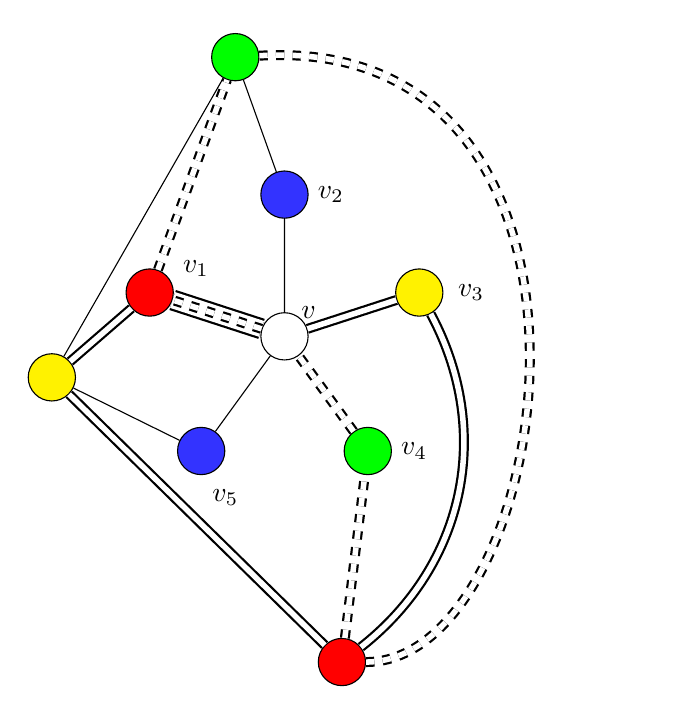
\begin{tikzpicture}[scale=.6,minimum size=6mm,inner sep=0pt]

% Draw center node and adjacent nodes
\foreach \name/\color/\theta in
    {A/yellow/18,B/blue!80/90,C/red/162,D/blue!80/234,E/green/306}
  \node[circle,draw,fill=\color] (\name) at (\theta:3) {};
\node[circle,draw] (O) at (0,0) {};
\node[above right]     at (O) {$v$};

\node[right,xshift=10pt] at (A) {$v_3$};
\node[right,xshift=8pt]  at (B) {$v_2$};
\node[above right,xshift=8pt]  at (C) {$v_1$};
\node[below right,yshift=-8pt] at (D) {$v_5$};
\node[right,xshift=8pt]  at (E) {$v_4$};

% Draw red-yellow path
\node[circle,draw,fill=yellow] (X1) at (-170:5) {};
\node[circle,draw,fill=red]    (X2) at (-80:7)  {};

\draw[thick,double distance=2pt] (A) -- (O);
\draw[thick,double distance=6pt] (O) -- (C);
\draw[thick,double distance=2pt] (C) --(X1) -- (X2);
\draw[thick,double distance=2pt,bend right=40] (X2) to (A);

% Draw red-green path
\node[circle,draw,fill=green] (Y1) at (100:6)  {};

\draw[dashed,thick,double distance=2pt] (O) -- (C) -- (Y1);
\draw[dashed,thick,double distance=2pt] 
  (Y1) .. controls (40:10) and (-50:9) .. (X2);
\draw[dashed,thick,double distance=2pt] (X2) -- (E) -- (O);

% Draw adjacent nodes
\draw (X1) -- (D) -- (O) -- (B) -- (Y1) -- (X1);

\end{tikzpicture}
\caption{לשרשארות אדום-צהוב ואדום-ירוק צמתים אדומים משותפים}
\label{f.five-kempe2}
\end{subfigure}
\hspace{3em}
\begin{subfigure}{.4\textwidth}
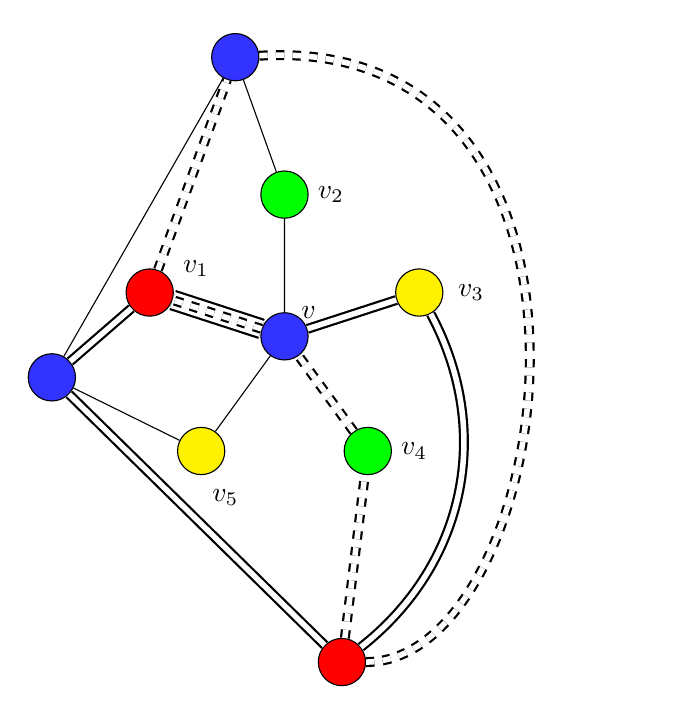
\begin{tikzpicture}[scale=.6,minimum size=6mm,inner sep=0pt]

% Draw center node and adjacent nodes
\foreach \name/\color/\theta in
    {A/yellow/18,B/green/90,C/red/162,D/yellow/234,E/green/306}
  \node[circle,draw,fill=\color] (\name) at (\theta:3) {};
\node[circle,draw,fill=blue!80] (O) at (0,0) {};
\node[above right]     at (O) {$v$};

\node[right,xshift=10pt] at (A) {$v_3$};
\node[right,xshift=8pt]  at (B) {$v_2$};
\node[above right,xshift=8pt]  at (C) {$v_1$};
\node[below right,yshift=-8pt] at (D) {$v_5$};
\node[right,xshift=8pt]  at (E) {$v_4$};


% Draw red-yellow path
\node[circle,draw,fill=blue!80] (X1) at (-170:5) {};
\node[circle,draw,fill=red]  (X2) at (-80:7)  {};

\draw[thick,double distance=2pt] (A) -- (O);
\draw[thick,double distance=6pt] (O) -- (C);
\draw[thick,double distance=2pt] (C) --(X1) -- (X2);
\draw[thick,double distance=2pt,bend right=40] (X2) to (A);

% Draw red-green path
\node[circle,draw,fill=blue!80] (Y1) at (100:6)  {};

\draw[dashed,thick,double distance=2pt] (O) -- (C) -- (Y1);
\draw[dashed,thick,double distance=2pt] 
  (Y1) .. controls (40:10) and (-50:9) .. (X2);
\draw[dashed,thick,double distance=2pt] (X2) -- (E) -- (O);

% Draw adjacent nodes
\draw (X1) -- (D) -- (O) -- (B) -- (Y1) -- (X1);
\end{tikzpicture}
\selectlanguage{hebrew}
\caption{החלפת הצבעים גורמת לצמתי הכחולים להיות קשורים}\label{f.five-kempe2-share}
\end{subfigure}
\end{center}
\end{figure}

\subsection*{מהי ההפתעה?}

משפט ארבעת הצבעים ידוע לשמצה, כי קל כל כך להציג אותו אבל קשה כל כך להוכיחו אותו. לכן מפתיע שההוכחה של משפט חמשת הצבעים כה פשוטה. החלק המרכזי של ההוכחה הוא משפט%
~\ref{thm.degree5}
(במפה מישורית חייב להיות צומת בדרגה
$5$
לכל היותר), שהוא משפט שאין  לו קשר עם צביעה. למעשה, הוא נובע מספירת צמתים וקשתות.

\subsection*{מקורות}
על משפט ארבעת הצבעים ראו 
\cite{thomas}, \cite{wiki:four}.
ההוכחה של משפט חמשת הצבעים לקוחה מ-%
\cite{thebook}, \cite{wiki:five}.
\cite{eppstein}
מביא הוכחות רבות לנוסחת אוילר.
השגיאה בהוכחה של קמפ
מתוארת ב-%
\cite{sipka}.
